%% Slide 10.
%\begin{frame}
%\begin{itemize}[<+->]
%\item
%Simulation has long been established as a useful method
%for inquiry into complex, ill-structured problem situations.
%\item
%One of its related fields is gaming, in which the tools are
%called simulation games.
%\item
%There is a \alert{need to develop an
%architecture} on which distributed simulation games can be
%built.
%\end{itemize}
%\end{frame}

%\subsection{Drivers for the Architecture}
\subsection{Drivers \& Requirements for the Architecture}

%% Slide 11.
\begin{frame}
\frametitle{Drivers for the Architecture}
\framesubtitle{Technology}
In order to understand the value of an architecture for gaming,
it is usefull first to focus on its drivers.
\pause
\begin{block}{}
Technology is considered to be the driver for
the development of a multi-player, distributed architecture
for gaming.
\end{block}
\pause
\vfill
\begin{block}{The question is:}
Why? To what extent have
the technological developments of the last decade improved
understanding and acceptance?
\end{block}
\end{frame}

%% Slide 12.
\begin{frame}
\frametitle{Drivers for the Architecture}
\framesubtitle{Why Technology?}
\begin{block}{The First Driver}
Incorporating state of the art web-enabled technologies
provides players with a simulated environment
which actually resembles the environment for which they are trained.
\end{block}
\pause
\begin{block}{A Second Driver}
Incorporating these technologies provides opportunities to construct a
more complex and realistic environment.
\end{block}
\pause
\begin{block}{A Third Driver}
Allows to embed algorithms for operational
decision making in simulation games.
\end{block}
\end{frame}


%\subsection{Requirements for the Architecture}

%% Slide 13.
\begin{frame}
\frametitle{Requirements for the Architecture}
\framesubtitle{The three U's}
When considering simulation games, there are three ``U'''s
that are important: the \alert{usefulness} of the tools and methods, their
\alert{usability}, and finally their \alert{usage}.
\end{frame}

%% Slide 14.
\begin{frame}
\frametitle{Requirements for the Architecture}
\framesubtitle{Usefulness \& Usability}
\begin{block}{Usefulness}
\begin{itemize}
\item <2->
Use simulated players to model players to increase complexity, or to increase
dynamics.
\item <3->
Depending on the complexity of the problem at hand,
it is useful to support long ($>$ 1 day) playing times.
\item <4->
Persistency of data and a
scenario service suitable for long time control are needed
to support long games.
\end{itemize}
\end{block}
\vfill
\begin{block}{Usability}<5->
User interfaces placed on top of generic services.
\end{block}
\end{frame}

%% Slide 15.
\begin{frame}
\frametitle{Requirements for the Architecture}
\framesubtitle{Usage \& Other Requirements}
\begin{block}{Usage}
\begin{itemize}
\item <2->
\alert{Scalability} is needed to support variable amounts of players.
\item <3->
\alert{Persistency} is needed to support the saving of data
when a (human) player is deliberately not on-line, or when
the connection with a player is unexpectedly lost.
\item <4->
Saving occurs at fixed and/or flexible points in time.
\end{itemize}
\end{block}
\begin{block}{Other Requirements}<5->
Other requirements are related to \alert{reliability}, \alert{robustness},
credibility and adaptivity.
\end{block}
\end{frame}

\subsection{An Architecture for Distribuited Games}

%% Slide 16.
\begin{frame}
\frametitle{An Architecture for Distribuited Games}
\framesubtitle{An Overview of the Architecture}
\begin{center}
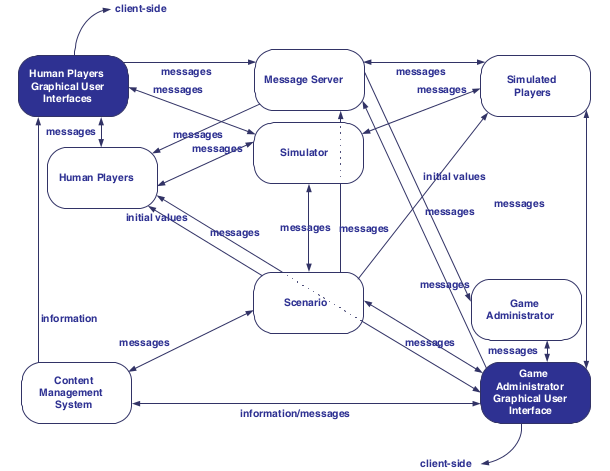
\includegraphics[scale=.85]{vanhouten.png}
\end{center}
\end{frame}

%% Slide 17.
\begin{frame}
\frametitle{An Architecture for Distribuited Games}
\framesubtitle{Technologies and Tools Used for Implementation}
\begin{itemize}[<+->]
\item
The reference implementation is a J2EE system which is
hosted on a JBOSS \& Tomcat combination.
\item
The simulation core was provided by the DSOL (Jacobs, Lang and Verbraeck
2002) suite for simulation which was accessed through RMI.
\item
A combination of HTML and JSP pages provided most of the
content to the actual players.
\item
Persistency of the game was
provided by MySQL and game scenarios were parsed from
locally accessible XML-files.
\item
The Java Message Service is
 used for the message service.
\end{itemize}
\end{frame}
